\assignment{2}{25/10}

\setcounter{question}{4}
\question For $\bm x = (x_1, x_2)$ and $\bm y = (y_1, y_2)$ in $\R^2$ define the \textbf{Jungle river metric} on $\R^2$ by
\[
    d(\bm x, \bm y) =
    \begin{cases}
        \lvert x_2 - y_2 \rvert & \text{if}\; x_1 = y_1, \\
        \lvert x_2 \rvert + \lvert y_2 \rvert + \lvert x_1 - y_1 \rvert & \text{if}\; x_1 \neq y_1.
    \end{cases}
\]
\begin{parts}
    \part Describe geometrically how $d$ measures the distance between two points in $\R^2$ and verify it is a metric.
    \begin{solution}
        For $(x_1, x_2), (y_1, y_2) \in \R^2$. When $x_1 \neq y_1$, our metric will will measure the length of the following path:
        \begin{enumerate}
            \item move to the first axis;
            \item move along until the second components are equal; then
            \item move back up to the point.
        \end{enumerate}
        The name comes from being trapped in a jungle that you cannot move along the $x$-axis through due to overgrowth, but you can move down to a river and travel along, then move back up. When $x_1 = y_1$, we have the standard metric on $\R^2$. Proving that this is a metric, let $\bm x, \bm y, \bm z \in \R^2$.
        \begin{enumerate}
            \item Positivity: 
                $d(\bm x, \bm y) \geq 0$ 
                clearly. When 
                $x_1 \neq y_1$, 
                we have that 
                $d(\bm x, \bm y) \neq 0$ 
                as 
                $\lvert x_1 - y_1 \rvert \neq 0$. 
                When 
                $x_1 = y_1$, $d(\bm x, \bm y) = 0 \iff x_2 = y_2 = 0$; 
                hence, 
                $d(\bm x, \bm y) = 0 \iff \bm x = \bm y$.

            \item Symmetry: it is clear that 
                $d(\bm x, \bm y) = d(\bm y, \bm x)$. 
                It follows from that fact that 
                $\lvert a - b \rvert = \lvert b - a \rvert$ 
                for all $a, b \in \R$.

            \item Triangle inequality: for
                $x_1 = y_1$
                this is just the typical triangle inequality. For
                $x_1 \neq y_1$:
                \begin{align*}
                    d(\bm x, \bm y) &=    \lvert x_2 \rvert + \lvert y_2 \rvert + \lvert x_1 - y_1 \rvert \\
                                    &\leq \lvert x_2 \rvert + \lvert z_2 \rvert + \lvert x_1 - z_1 \rvert
                                    + \lvert z_2 \rvert + \lvert y_2 \rvert + \lvert z_1 - y_1 \rvert \\
                                    &=    d(\bm x, \bm z) + d(\bm z, \bm y).
                \end{align*}
        \end{enumerate}
        Hence, $d$ is a metric over $\R^2$.
    \end{solution}

    \part Sketch the open balls $B_1(\bm 0)$ and $B_2((3, 1))$ in $\R^2$ withg respect to this metric.
    \begin{solution}
        \begin{center}
            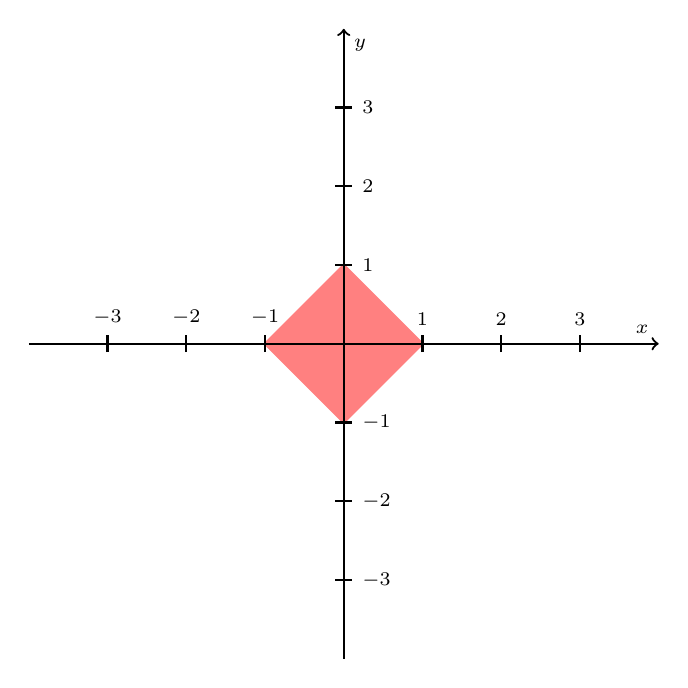
\begin{tikzpicture}
                \begin{scope}[thick,font=\scriptsize]
                    \draw [thick, color=red!50, fill=red!50] (0,1) -- (1,0) -- (0, -1) -- (-1, 0) -- cycle;
                    \draw [->] (-4,0) -- (4,0) node [above left]  {$x$};
                    \draw [->] (0,-4) -- (0,4) node [below right] {$y$};
                    
                    \foreach \n in {-3,...,-1,1,2,...,3}{%
                        \draw (\n,-3pt) -- (\n,3pt)   node [above] {$\n$};
                        \draw (-3pt,\n) -- (3pt,\n)   node [right] {$\n$};}
                \end{scope}
            \end{tikzpicture}
        \end{center}
        \begin{center}
            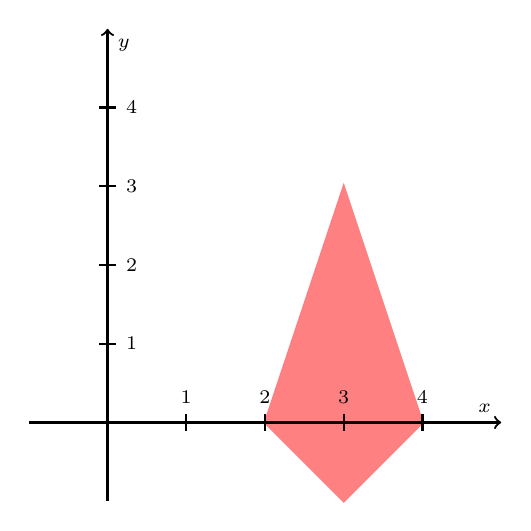
\begin{tikzpicture}
                \begin{scope}[thick,font=\scriptsize]
                    \draw [thick, color=red!50, fill=red!50] (2,0) -- (3,3) -- (4,0) -- (3,-1) -- cycle;
                    \draw [->] (-1,0) -- (5,0) node [above left]  {$x$};
                    \draw [->] (0,-1) -- (0,5) node [below right] {$y$};
                    
                    \foreach \n in {1,2,...,4}{%
                        \draw (\n,-3pt) -- (\n,3pt)   node [above] {$\n$};
                        \draw (-3pt,\n) -- (3pt,\n)   node [right] {$\n$};}
                \end{scope}
            \end{tikzpicture}
        \end{center}
    \end{solution}
\end{parts}

\setcounter{question}{6}
\question
\begin{parts}
    \part Show that in any metric space $(X, d)$ the set $\{x\}$, consisting of a single point $x \in X$, is closed.
    \begin{solution}
        Consider $X \setminus \{x\}$. This is open as $\forall y \in X \setminus \{x\}$ there exists $\varepsilon > 0$ such that $B_\varepsilon(y) \subset X \setminus \{ x \}$. Hence, $\{ x \}$ is closed.
    \end{solution}

    \part Show that in any metric space $(X, d)$ the closed ball $\bar B_r(x) = \{y \in X: d(y, x) \leq r\}$, of radius $r > 0$ centred at $x \in X$, is closed.
    \begin{solution}
        Consider the closed ball 
        $\bar B_r(x)$ 
        for some 
        $x \in X$. 
        Now consider a
        $y \in X \setminus \bar B_r(x)$.
        Let 
        $\varepsilon = d(x, y) - r$
        and 
        $z \in B_\varepsilon(y)$.
        Then
        \begin{align*}
            d(x, y) &\leq d(x, z) + d(z, x)     \\
                    &<    d(x, z) + \varepsilon \\
            d(x, z) &>    d(x, y) - \varepsilon \\
                    &=    d(x, y) - d(x, y) + r \\
                    &=    r;
        \end{align*}
        hence, 
        $B_\varepsilon(y) \not\subset B_r(x) \implies B_\varepsilon(y) \subset X \setminus \bar B_r(x)$
        and so 
        $X \setminus \bar B_r(x)$
        is open; therefore
        $\bar B_r(x)$
        is closed.
    \end{solution}
\end{parts}

\setcounter{question}{9}
\question Let $(X, d)$ be a metric space. Show that $X$ is \textbf{Hausdorff}; that is, for any pair of distinct points $x$ and $y$ in $X$ there exists open sets $U$ and $V$ such that $x \in U$, $y \in V$, and $U \cap V = \emptyset$.
\begin{solution}
    For $x$ and $y$ we consider the balls $B_{\lvert x - y \rvert}(x)$ and $B_{\lvert x - y \rvert}(y)$. As we know that open balls are open sets and they do not intersect (and they obviously contain $x$ and $y$ respectively), this meets the requirements for $X$ being Hausdorff.
\end{solution}

\setcounter{question}{14}
\question Show that if a sequence $\{x_n\}$ converges in a discrete metric space, then it is eventually constant.
\begin{solution}
    We know that $x_n \to x$ as $n \to \infty$, that is
    \[ \forall\; \varepsilon > 0 \;\exists\; N \in \N \;\forall\; n \geq N: d(x_n, x) < \varepsilon. \]
    Let $\varepsilon = 1$, then for some $N \in \N$, $d(x_n, x) < 1$ for all $n \geq N$. That is, $d(x_n , x) = 0$ and hence $x_n = x$; constant.
\end{solution}
